\documentclass[UTF8, fontset=ubuntu]{ctexart}
\usepackage{parskip}
\usepackage{tikz}
\usepackage{amssymb}
\usetikzlibrary{datavisualization.formats.functions}
\def\mytypesetter#1{%
\pgfmathparse{#1/pi}%
\pgfmathprintnumber{\pgfmathresult}$\pi$%
}
\begin{document}
1.导数与反函数\\
如果$f$在其定义域$(a,b)$上可导且满足以下条件中的任意一条:\\
(1)对于所有的在$(a,b)$中的$x$, $f'(x)>0$;\\
(2)对于所有的在$(a,b)$中的$x$, $f'(x)<0$;\\
(3)对于所有的在$(a,b)$中的$x$, $f'(x)\geqslant 0$且对于有限个数的$x$, $f'(x)=0$;\\
(4)对于所有的在$(a,b)$中的$x$, $f'(x)\leqslant 0$且对于有限个数的$x$, $f'(x)=0$.\\
则$f$有反函数.\\[2ex]

2.反函数的导数\\[1ex]
\framebox{如果$\displaystyle y=f^{-1}(x)$, 则$\displaystyle\frac{dy}{dx}=\frac{1}{f'(y)}=\frac{1}{f'(f^{-1}(x))}$}\\[1ex]
** $f(y)$是将$f(x)$中的$x$替换为$y$的版本, $f'(y)$类似.\\[2ex]

3.反三角函数\\
(1)$\sin^{-1}$是奇函数; 其定义域为$[-1,1]$, 值域为$\displaystyle[-\frac{\pi}{2},\frac{\pi}{2}]$\\[1ex]
(2)$\displaystyle\frac{d}{dx}\sin^{-1}(x)=\frac{1}{\sqrt{1-x^2}}$, 其中$-1<x<1$.\\[1ex]
\begin{center}
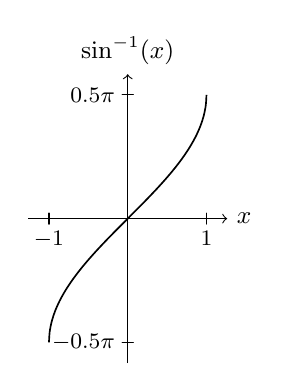
\begin{tikzpicture}
\datavisualization[school book axes, visualize as smooth line, y axis={ticks={step=(pi/2), major={at={(-pi/2),(pi/2)}}, tick typesetter/.code=\mytypesetter{##1}}, label=$\sin^{-1}(x)$}, x axis={label=$x$}]
data[format=function]{
	var y : interval [-pi/2:pi/2];
	func x = sin(\value{y} r);
};
\end{tikzpicture}\\[1ex]
\end{center}
(3)$\cos^{-1}$既不是偶函数也不是奇函数; 其定义域为$[-1,1]$, 值域为$[0,\pi]$.\\[1ex]
(4)$\displaystyle\frac{d}{dx}\cos^{-1}(x)=-\frac{1}{\sqrt{1-x^2}}$, 其中$-1<x<1$.\\[1ex]
\begin{center}
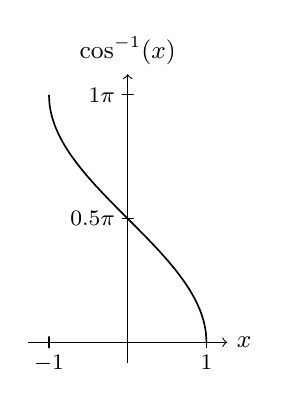
\begin{tikzpicture}
\datavisualization[school book axes, visualize as smooth line, y axis={ticks={step=(pi/2), major={at={(pi/2),(pi)}}, tick typesetter/.code=\mytypesetter{##1}}, label=$\cos^{-1}(x)$}, x axis={label=$x$}]
data[format=function]{
	var y : interval [0:pi];
	func x = cos(\value{y} r);
};
\end{tikzpicture}\\[1ex]
\end{center}
(5)$\tan^{-1}$是奇函数; 其定义域是$\mathbb{R}$且值域是$\displaystyle(-\frac{\pi}{2},\frac{\pi}{2})$.\\[1ex]
(6)对于所有的实数$x$, $\displaystyle\frac{d}{dx}\tan^{-1}(x)=\frac{1}{1+x^2}$.\\[1ex]
\begin{center}
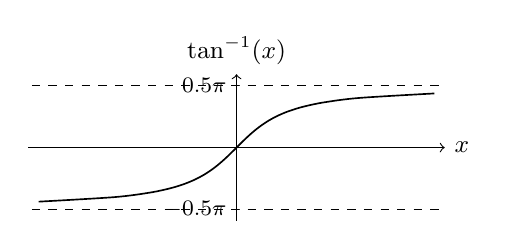
\begin{tikzpicture}[scale=0.5]
\datavisualization[school book axes, visualize as smooth line, y axis={ticks={step=(pi/2), major={at={(-pi/2),(pi/2)}}, tick typesetter/.code=\mytypesetter{##1}}, include value={-1.6,1.6}, label=$\tan^{-1}(x)$}, x axis={ticks=none, label=$x$}]
data[format=function]{
    var y : interval [-pi*7/16:pi*7/16];
    func x = tan(\value{y} r);
};
\draw[dashed] (-5.2, pi/2) -- (5.2, pi/2);
\draw[dashed] (-5.2, -pi/2) -- (5.2, -pi/2);
\end{tikzpicture}\\[1ex]
\end{center}
(7)$\cot^{-1}$既不是奇函数也不是偶函数; 其定义域为$\mathbb{R}$且值域是$(0,\pi)$\\[1ex]
(8)对于所有的实数$x$, $\displaystyle\frac{d}{dx}\cot^{-1}(x)=-\frac{1}{1+x^2}$.\\[1ex]
\begin{center}
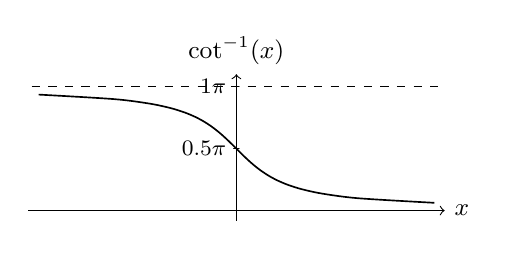
\begin{tikzpicture}[scale=0.5]
\datavisualization[school book axes, visualize as smooth line, y axis={ticks={step=(pi/2), major={at={(pi/2),(pi)}}, tick typesetter/.code=\mytypesetter{##1}}, include value={3.2}, label=$\cot^{-1}(x)$}, x axis={ticks=none, label=$x$}]
data[format=function]{
    var y : interval [pi*1/16:pi*15/16];
    func x = cot(\value{y} r);
};
\draw[dashed] (-5.2, pi) -- (5.2, pi);
\end{tikzpicture}
\end{center}
(9)$\sec^{-1}$既不是奇函数也不是偶函数; 其定义域是$(-\infty,-1]\cup[1,\infty)$且值域是$\displaystyle[0,\frac{\pi}{2})\cup(\frac{\pi}{2},\pi]$.\\[1ex]
(10)对于$x>1$或$x<-1$, $\displaystyle\frac{d}{dx}\sec^{-1}(x)=\frac{1}{|x|\sqrt{x^2-1}}$.\\[1ex]
\begin{center}
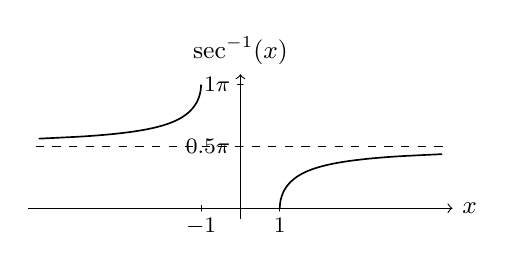
\begin{tikzpicture}[scale=0.5]
\datavisualization[school book axes, visualize as smooth line/.list={sec1, sec2}, y axis={ticks={step=(pi/2), major={at={(pi/2),(pi)}}, tick typesetter/.code=\mytypesetter{##1}}, label=$\sec^{-1}(x)$}, x axis={ticks={major={at={-1,0,1}}}, label=$x$}]
data [set=sec1, format=function] {
var y : interval [0:pi*7/16];
func x = 1/cos(\value y r);
}
data [set=sec2,format=function] {
var y : interval [pi*9/16:pi];
func x = 1/cos(\value y r);
};
\draw[dashed] (-5.2, 0.5*pi) -- (5.2, 0.5*pi);
\end{tikzpicture}
\end{center}
(11)$\csc^{-1}$是奇函数; 其定义域为$(-\infty,-1]\cup[1,\infty)$且值域是$\displaystyle[-\frac{\pi}{2},0)\cup(0,\frac{\pi}{2}]$.\\[1ex]
(12)对于$x>1$或$x<-1$, $\displaystyle\frac{d}{dx}\csc^{-1}(x)=-\frac{1}{|x|\sqrt{x^2-1}}$.\\[2ex]
\begin{center}
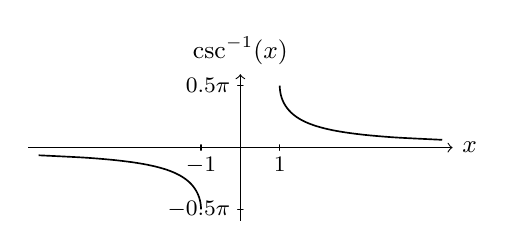
\begin{tikzpicture}[scale=0.5]
\datavisualization[school book axes, visualize as smooth line/.list={csc1, csc2}, y axis={ticks={step=(pi/2), major={at={(-pi/2),(pi/2)}}, tick typesetter/.code=\mytypesetter{##1}}, include value={-1.6,1.6}, label=$\csc^{-1}(x)$}, x axis={ticks={major={at={-1,0,1}}}, label=$x$}]
data [set=csc1, format=function] {
var y : interval [pi*1/16:pi/2];
func x = 1/sin(\value y r);
}
data [set=csc2,format=function] {
var y : interval [-pi/2:-pi*1/16];
func x = 1/sin(\value y r);
};
\end{tikzpicture}
\end{center}\vspace{2ex}

4.计算反三角函数\\
化简形如$\sin^{-1}(\sin(\alpha))$的三角函数:\\
\phantom{(1)}获取指定角$\alpha$的参照角\\
\phantom{(1)}找到反三角函数定义域中拥有该参照角的角\\
\phantom{(1)}确定该角的正弦值与$\alpha$参照角的正弦值符号一致\\[2ex]

5.反双曲函数\\
(1)$\sinh^{-1}$是奇函数; 其定义域和值域都是$\mathbb{R}$.\\[1ex]
(2)对于所有的实数$x$, $\displaystyle\frac{d}{dx}\sinh^{-1}(x)=\frac{1}{\sqrt{x^2+1}}$.\\[1ex]
(3)$\cosh^{-1}$既不是奇函数也不是偶函数; 其定义域是$[1,\infty)$且值域是$[0,\infty)$.\\[1ex]
(4)对于$x>1$, $\displaystyle\frac{d}{dx}\cosh^{-1}(x)=\frac{1}{\sqrt{x^2-1}}$.\\[1ex]
\end{document}
